\section{App utenti}

\subsection{Introduzione e scopo del prodotto}
L'applicazione mobile è sviluppata per due diverse tipologie di utente ovvero il dipendente e l'addetto alle pulizie.

In generale offre all'utente le seguenti funzionalità:
\begin{itemize}
	\item \textbf{Login:} l'utente ha la possibilità di autenticarsi inserendo il proprio username e password; \\
	\item \textbf{Logout:} l'utente ha la possibilità di deautenticarsi premendo sull'elemento della lista "Logout" del menù principale in alto a destra. \\
\end{itemize}

Per quanto riguarda il dipendente, l'applicazione offre i seguenti servizi:
\begin{itemize}
	\item \textbf{Scansione:} il dipendente ha la possibilità di scansionare una \glock{postazione} per poter visualizzare lo stato di essa e altre informazioni come le prenotazioni associate a essa; \\
	\item \textbf{Occupazione:} il dipendente dopo aver scansionato una postazione può occuparla se questa è prenotata da lui o è libera e igienizzata; \\
	\item \textbf{Igienizzazione:} il dipendente dopo aver scansionato una postazione la può igienizzare se questa risulta non igienizzata; \\
	\item \textbf{Lista prenotazioni:} il dipendente può visualizzare le prenotazioni effettuate premendo sull'elemento della lista "Visualizza prenotazioni" del menù principale in alto a destra; \\
	\item \textbf{Disdetta prenotazione:} il dipendente può disdire una prenotazione dopo che è entrato nella pagina in cui visualizza tutte le prenotazioni effettuate; \\
	\item \textbf{Guida:} il dipendente può visualizzare la guida premendo sull'elemento della lista "Guida" del menù principale in alto a destra; \\
	\item \textbf{Prenotazione postazione:} il dipendente può prenotare una postazione premendo sull'elemento della lista "Prenota postazione" del menù principale in alto a destra.
	Dopo aver premuto dovrà inserire la data, l'ora di inizio, l'ora di fine e la stanza.
	Una volta premuto sul bottone "Cerca", l'utente visualizzerà tutte le postazioni disponibili nella stanza, nel range orario e nella data inseriti e potrà decidere di effettuare una prenotazione. \\	
\end{itemize}

Per quanto riguarda l'addetto alle pulizie, l'applicazione offre i seguenti servizi:
\begin{itemize}
	\item \textbf{Lista postazioni:} l'addetto alle pulizie può visualizzare tutte le postazioni da igienizzare premendo sul bottone "Ottieni postazioni", presente nella pagina principale; \\
	\item \textbf{Lista stanze:} l'addetto alle pulizie può visualizzare tutte le stanze da igienizzare premendo sul bottone "Ottieni stanze", presente nella pagina principale; \\
	\item \textbf{Igienizzazione postazioni:} l'addetto alle pulizie può igienizzare le postazioni e segnalare questa azione premendo sul bottone "Igienizza" presente sulla destra di ogni postazione;
	\item \textbf{Igienizzazione stanze:} l'addetto alle pulizie può igienizzare le stanze e segnalare questa azione premendo sul bottone "Igienizza" presente sulla destra di ogni stanza;
	\item \textbf{Guida:} l'addetto alle pulizie può visualizzare la guida premendo sull’elemento della lista "Guida" del menù principale in alto a destra; \\
	
\end{itemize}

\subsection{Requisiti e installazione}
	Per il corretto funzionamento l'applicazione mobile richiede di essere installata su un dispositivo con sistema operativo \glock{Android} con versione uguale o superiore alla 6.0 Marshmallow.
	
	\subsection{Utilizzo applicazione per i dipendenti}
	L'applicazione mobile viene utilizzata dagli utenti che vogliono accedere a una postazione di una stanza dell'\glock{organizzazione}. Essi hanno la possibilità di effettuare una prenotazione e di conoscere lo stato di una postazione, tramite la scansione del \glock{tag NFC} associato. Inoltre per ogni occupazione viene registrato l'orario di inizio e di fine, e monitorata la presenza in \glock{tempo reale} da parte dell'amministratore. Inoltre, ogni utente ha la possibilità di effettuare un'igienizzazione di una postazione precedentemente utilizzata. 
	\\All'utente dell'applicazione vengono offerte tutte le funzionalità indicate in questa sezione.
	\subsubsection{Login}
	\begin{figure}[H]
		\centering
		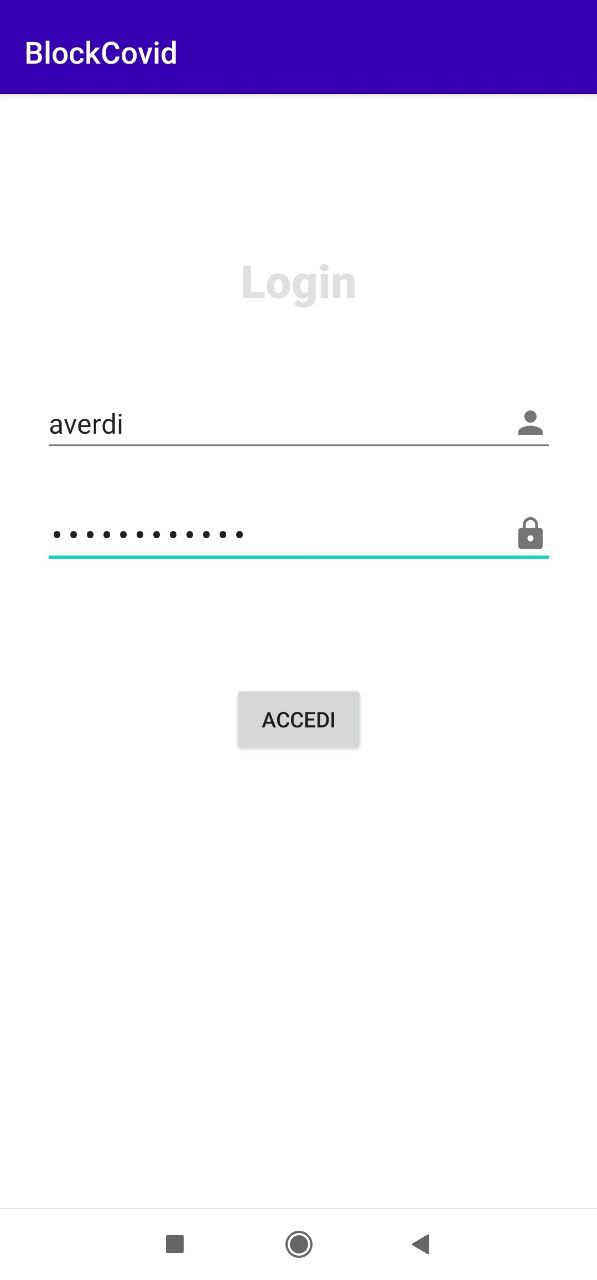
\includegraphics[width=5cm]{res/images/loginDipendente.png}
		\caption{Login utente}
	\end{figure}
	L'utente può autenticarsi nella pagina del login inserendo il proprio username e la propria password nelle caselle di testo corrispondenti.
	Nel caso in cui inserisca le credenziali corrette otterrà l'accesso all'applicazione e quindi alla pagina principale, altrimenti verrà visualizzato un messaggio di errore.
	\begin{figure}[H]
		\centering
		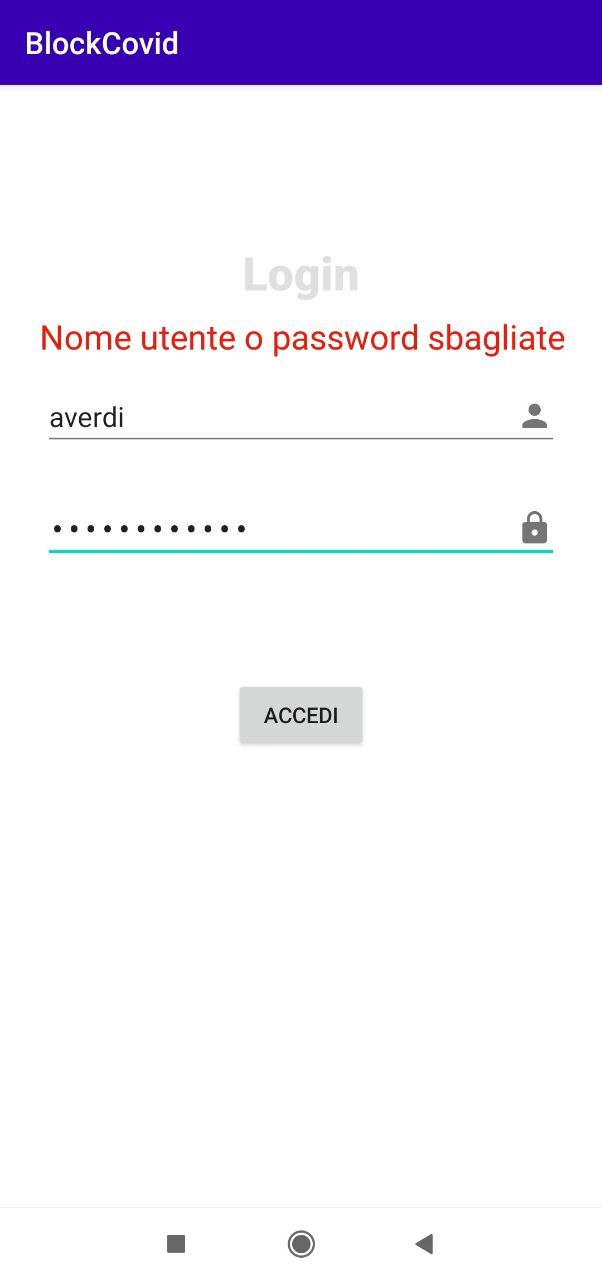
\includegraphics[width=5cm]{res/images/credenzialiErrate.png}
		\caption{Inserimento credenziali errate}
	\end{figure}
	
	\subsubsection{Logout}
	\begin{figure}[H]
		\centering
		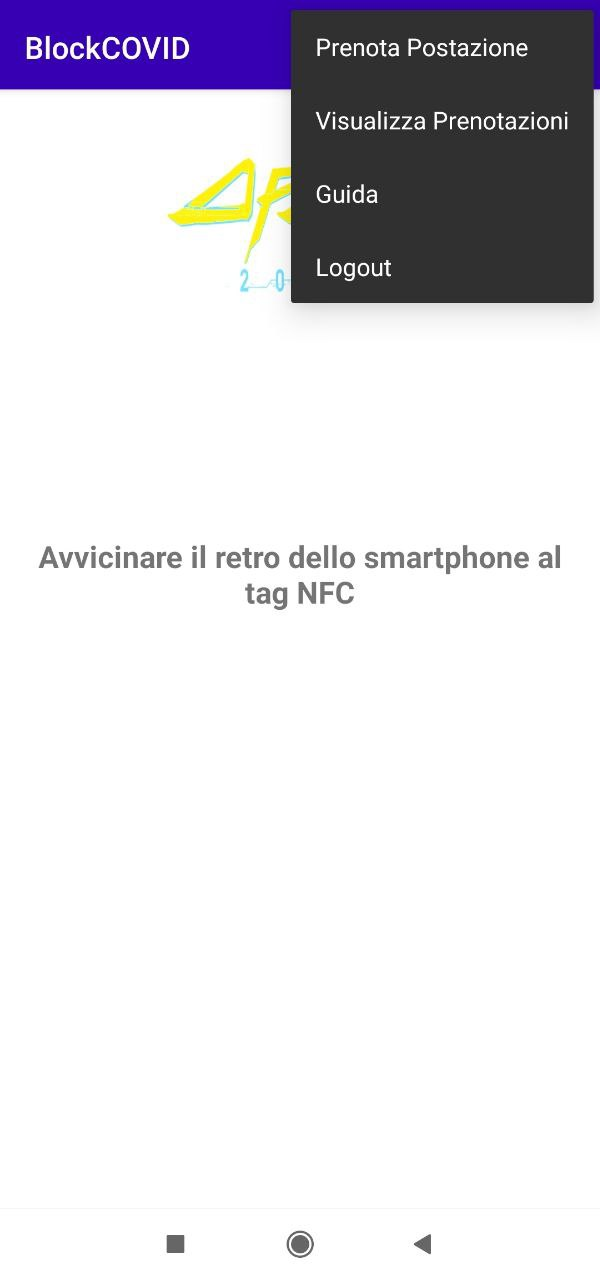
\includegraphics[width=5cm]{res/images/menuATendina.png}
		\caption{Logout utente}
	\end{figure}
	L'utente può eseguire il logout aprendo il menù a tendina in alto a destra e poi cliccando su logout. Avvenuta questa operazione l'utente sarà deautenticato dal sistema e si troverà nella pagina del login.
	
	\subsubsection{Scansione tag NFC}
	\begin{figure}[H]
		\centering
		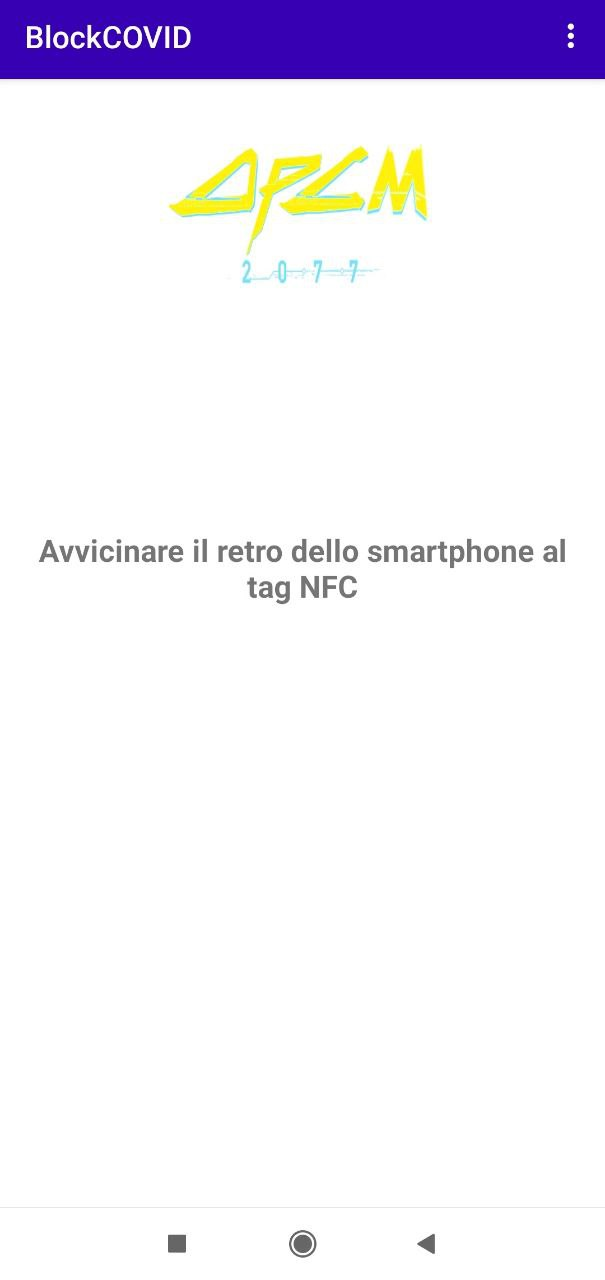
\includegraphics[width=5cm]{res/images/avvicinaSmartphone.png}
		\caption{Scansione tagNFC}
	\end{figure}
	L'utente si trova nella pagina principale dell'applicazione e gli viene chiesto di effettuare una scansione del tag NFC tramite lo smartphone per ottenere tutte le informazioni sulla postazione.
	\subsubsection{Visualizzazione stato postazione}
	\begin{figure}[H]
		\centering
		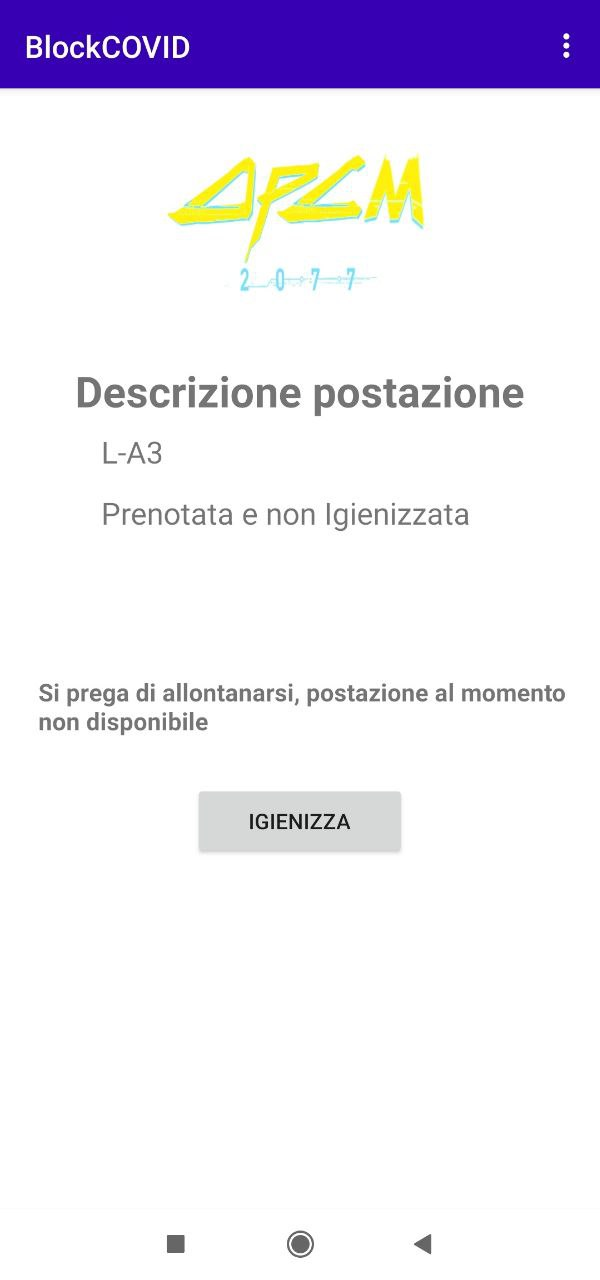
\includegraphics[width=5cm]{res/images/prenotataENonIgienizzata.png}
		\caption{Stato postazione}
	\end{figure}
	L'utente ha effettuato la scansione di una postazione e riceve le seguenti informazioni nella pagina principale dell'applicazione:
	\begin{itemize}
		\item nome postazione;
		\item stato postazione.
	\end{itemize}
	In base allo stato in cui si trova la postazione, l'utente visualizzerà un messaggio differente:
	\begin{itemize}
		\item se libera e igienizzata, si invita l'utente a indicare il numero di ore per cui intende effettuare un'occupazione della postazione;
		\item se libera e non igienizzata, si invita l'utente a effettuare la pulizia autonoma della postazione tramite il kit aziendale e quindi di cliccare il bottone "igienizza", che modificherà lo stato in igienizzata;
		\item se prenotata dallo stesso utente e igienizzata, viene mostrato un messaggio contenente la data e ora di inizio e fine della prenotazione e si invita l'utente a indicare il numero di ore per cui intende effettuare l'occupazione della postazione;
		\item se prenotata da un altro utente e igienizzata, si invita l'utente ad abbandonare la postazione dato che al momento non è disponibile;
		\item se prenotata e non igienizzata, si invita l'utente a effettuare la pulizia autonoma della postazione tramite il kit aziendale e quindi di cliccare il bottone "igienizza", che modificherà lo stato in prenotata e igienizzata;
		\item se guasta e igienizzata, si invita l'utente ad abbandonare la postazione dato che al momento non è disponibile;
		\item se guasta e non igienizzata, si invita l'utente a effettuare la pulizia autonoma della postazione tramite il kit aziendale e quindi di cliccare il bottone "igienizza", che modificherà lo stato in guasta e igienizzata.
	\end{itemize}
	
	\subsubsection{Occupazione postazione}
	\begin{figure}[H]
		\centering
		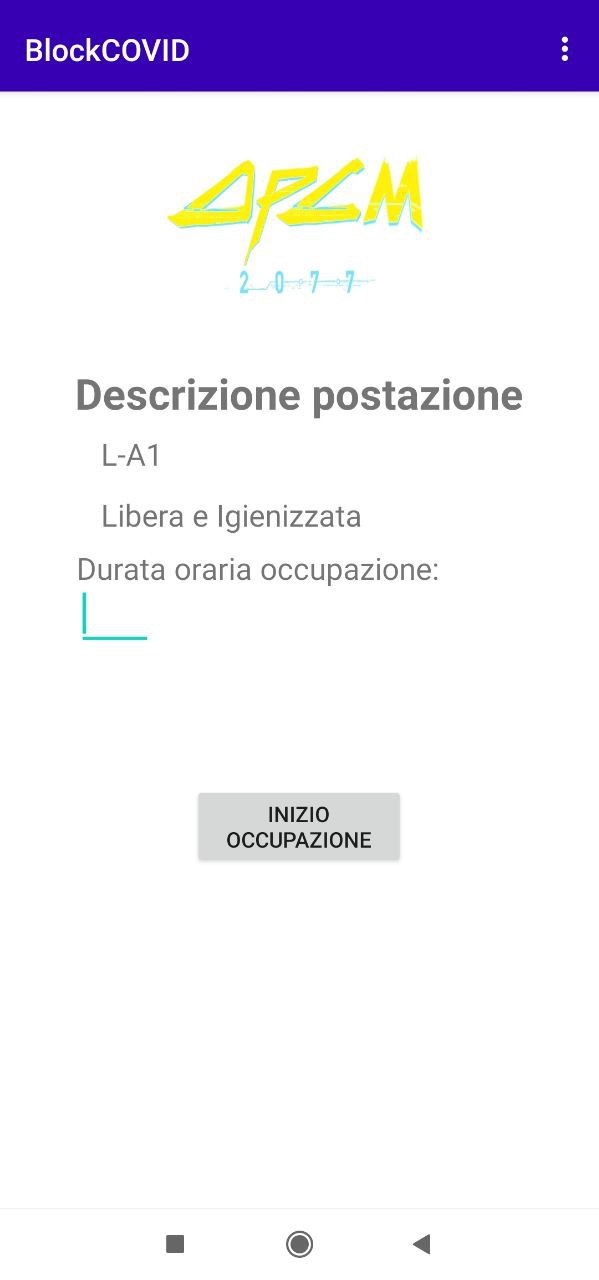
\includegraphics[width=5cm]{res/images/inizioOccupazione.png}
		\caption{Inizio occupazione postazione}
	\end{figure}
	L'utente dopo aver scansionato con il proprio smartphone il tag NFC, può occupare la postazione per un determinato numero di ore da lui selezionato. Lo stato della postazione deve essere libera e igienizzata o prenotata dallo stesso utente.
	\begin{figure}[H]
		\centering
		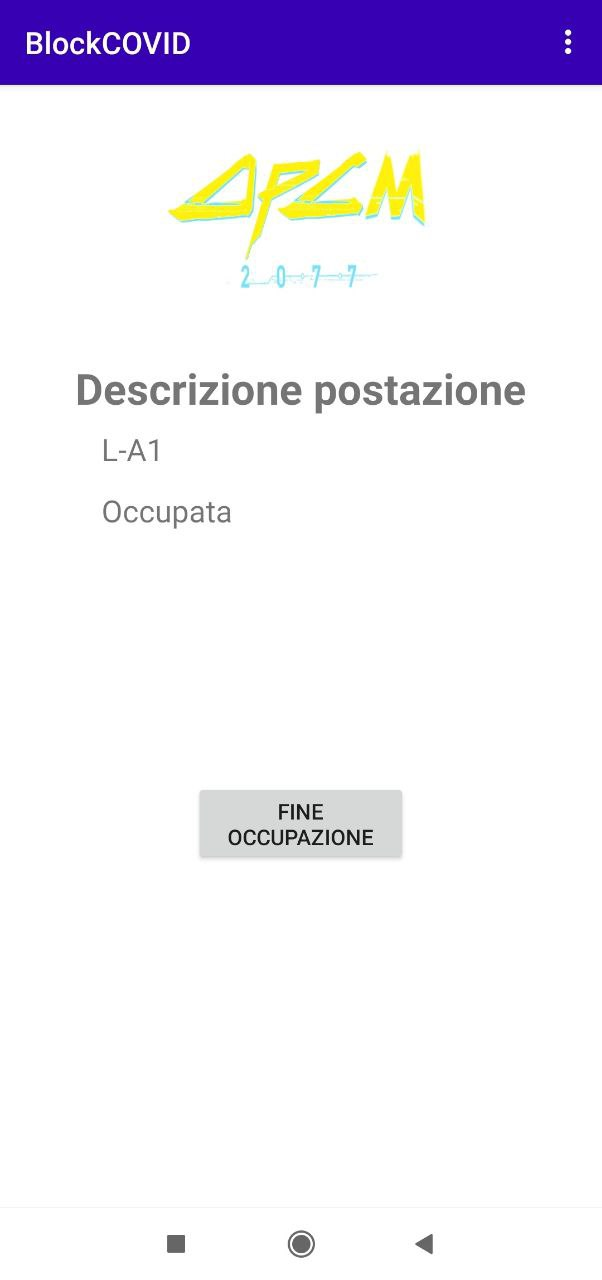
\includegraphics[width=5cm]{res/images/occupata.png}
		\caption{Fine occupazione postazione}
	\end{figure}
	Una volta avvenuta con successo l'occupazione, lo stato della postazione diventa "Occupato" e da quel momento in poi risulta possibile terminare l'occupazione premendo il bottone "Fine Occupazione".
	\subsubsection{Igienizzazione postazione}
	\begin{figure}[H]
		\centering
		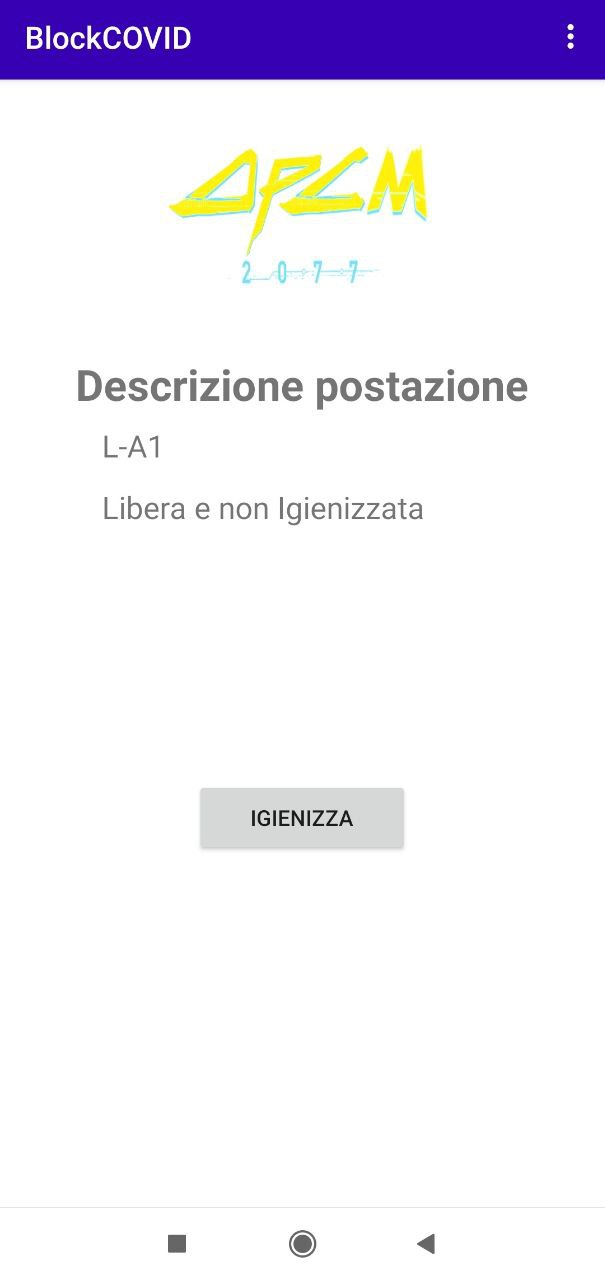
\includegraphics[width=5cm]{res/images/liberaENonIgienizzata.png}
		\caption{Igienizzazione postazione}
	\end{figure}
	L'utente igienizza una postazione il cui stato è diverso da "igienizzato" e lo segnala premendo l'apposito bottone "igienizza" nella pagina principale dell'applicazione. In modo automatico lo stato della postazione viene registrato come libera e igienizzata, prenotata e igienizzata o guasta e igienizzata.
	\subsubsection{Visualizzazione lista prenotazioni}
	\begin{figure}[H]
		\centering
		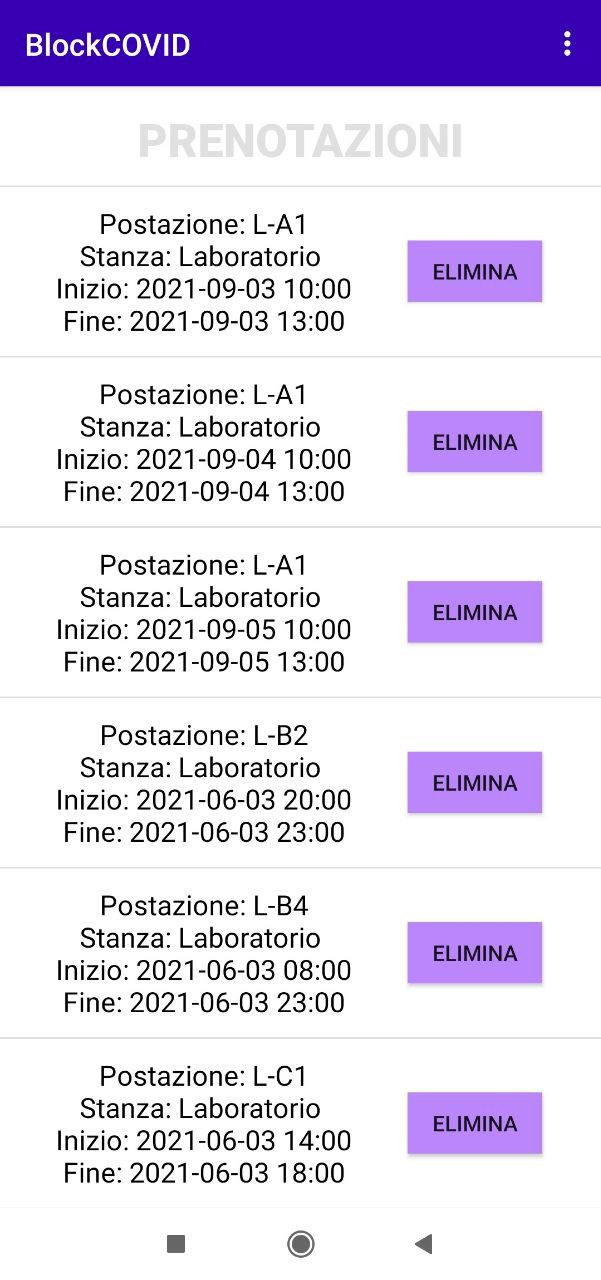
\includegraphics[width=5cm]{res/images/listaPrenotazioni.png}
		\caption{Visualizzazione lista prenotazioni}
	\end{figure}
	L’utente può accedere alla sezione per la visualizzazione della lista delle prenotazioni da lui effettuate cliccando nel menù a tendina in alto a destra "Visualizza prenotazioni".
	Ogni prenotazione mostra le seguenti informazioni:
	\begin{itemize}
		\item nome della postazione;
		\item nome della stanza;
		\item data e ora di inizio;
		\item data e ora di fine.
	\end{itemize}
	\subsubsection{Disdetta prenotazione}
	\begin{figure}[H]
		\centering
		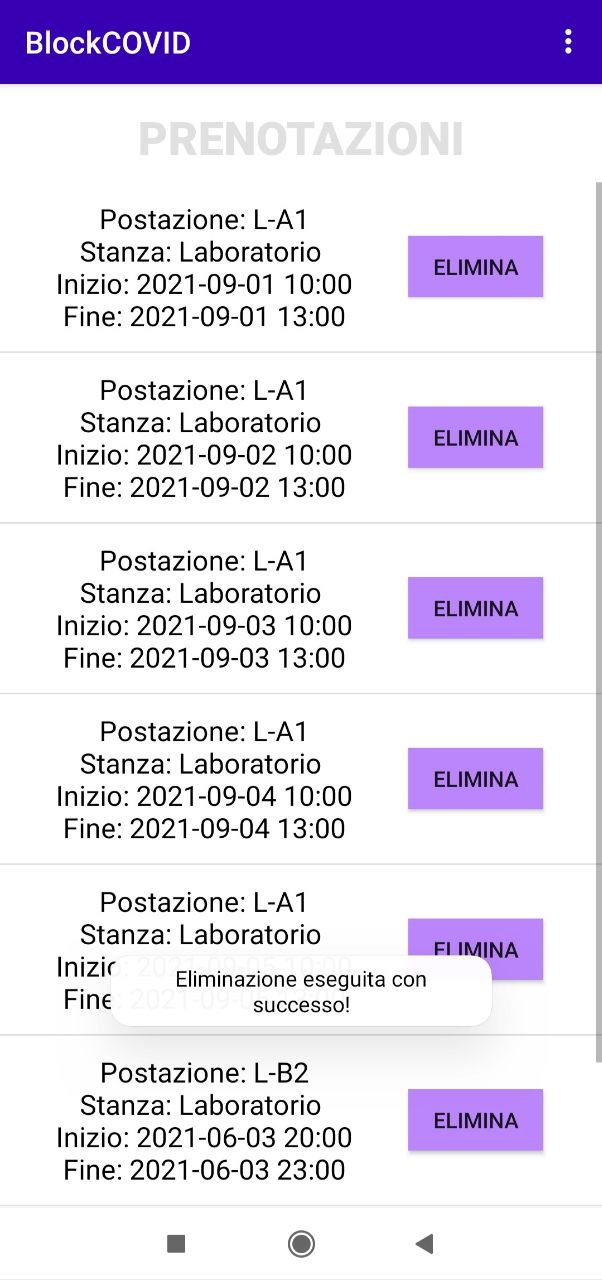
\includegraphics[width=5cm]{res/images/MessaggioEliminazioneAvvenutaSuccesso.png}
		\caption{Disdetta prenotazione}
	\end{figure}
	L’utente si trova nella sezione di visualizzazione della lista delle prenotazioni, arrivatoci cliccando il menù a tendina in alto a destra, e disdice una prenotazione da lui effettuata in precedenza premendo il bottone "Elimina". A seguito di tale azione la prenotazione non viene più visualizzata nella lista e compare il messaggio "Eliminazione eseguita con successo!".
	\subsubsection{Guida utente}
	\begin{figure}[H]
		\centering
		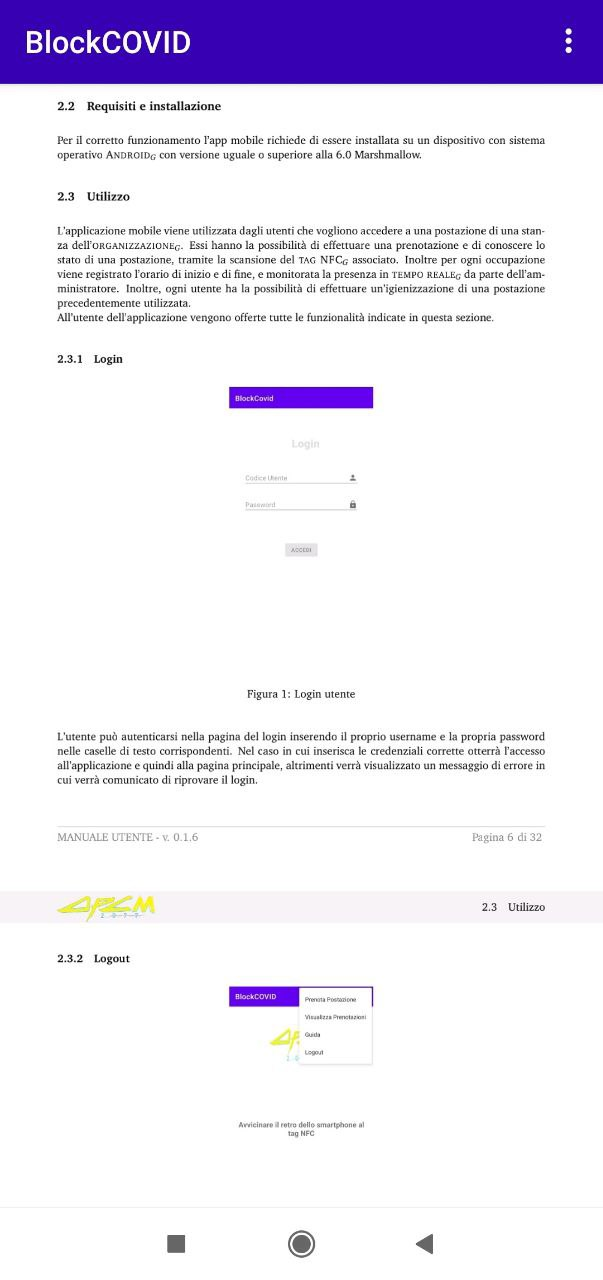
\includegraphics[width=5cm]{res/images/guidaDipendente.png}
		\caption{Guida dipendente}
	\end{figure}
	L’utente accede alla pagina "Guida utente", cliccando la sezione apposita del menù a tendina in alto a destra, e riceve una guida riguardo le funzionalità principali dell'applicazione.
	\subsubsection{Prenotazione postazione}
	\begin{figure}[H]
		\centering
		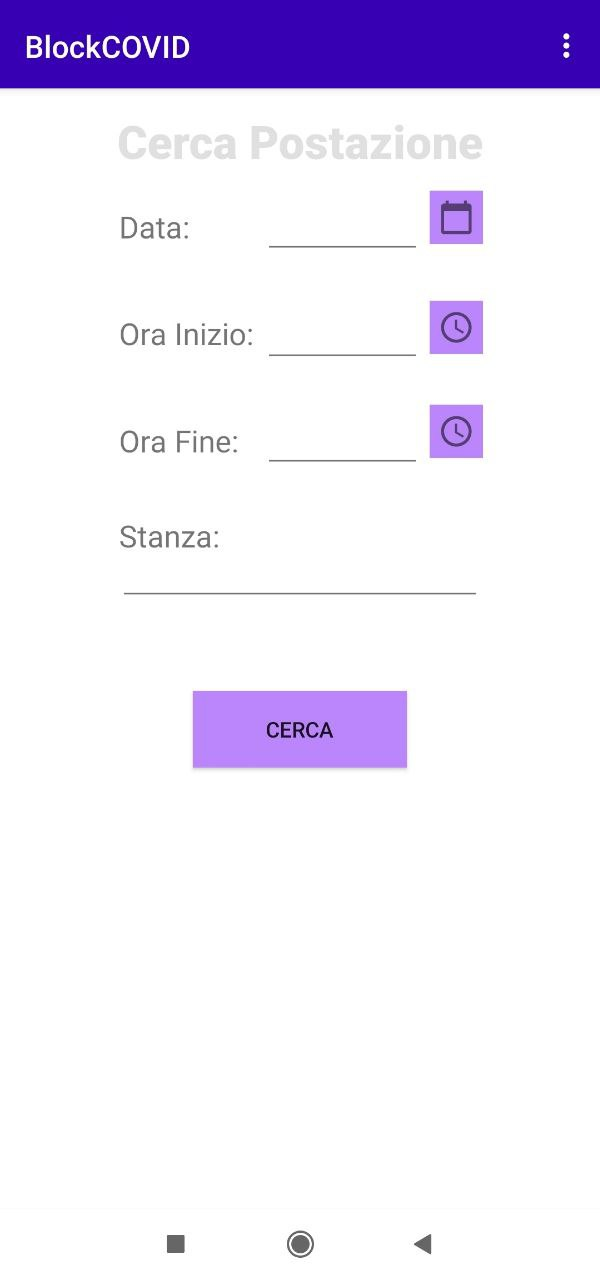
\includegraphics[width=5cm]{res/images/cerca.png}
		\caption{Inserimento campi di ricerca}
	\end{figure}
	Il dipendente può prenotare una postazione premendo sull'elemento della lista "Prenota postazione" del menù principale in alto a destra.
	Dopo aver premuto dovrà inserire la data, l'ora di inizio, l'ora di fine e la stanza obbligatoriamente. Per facilitare l'utente nell'inserimento dei dati, sono presenti una vista a calendario per la selezione di una data e una vista a orologio per la selezione di un orario. Una volta premuto sul bottone "Cerca", l’utente visualizzerà tutte le postazioni disponibili nella stanza, nel range orario e nella data inseriti e potrà decidere di effettuare una prenotazione premendo il bottone "Prenota" presente sulla destra di ogni postazione.
	\begin{figure}[H]
		\centering
		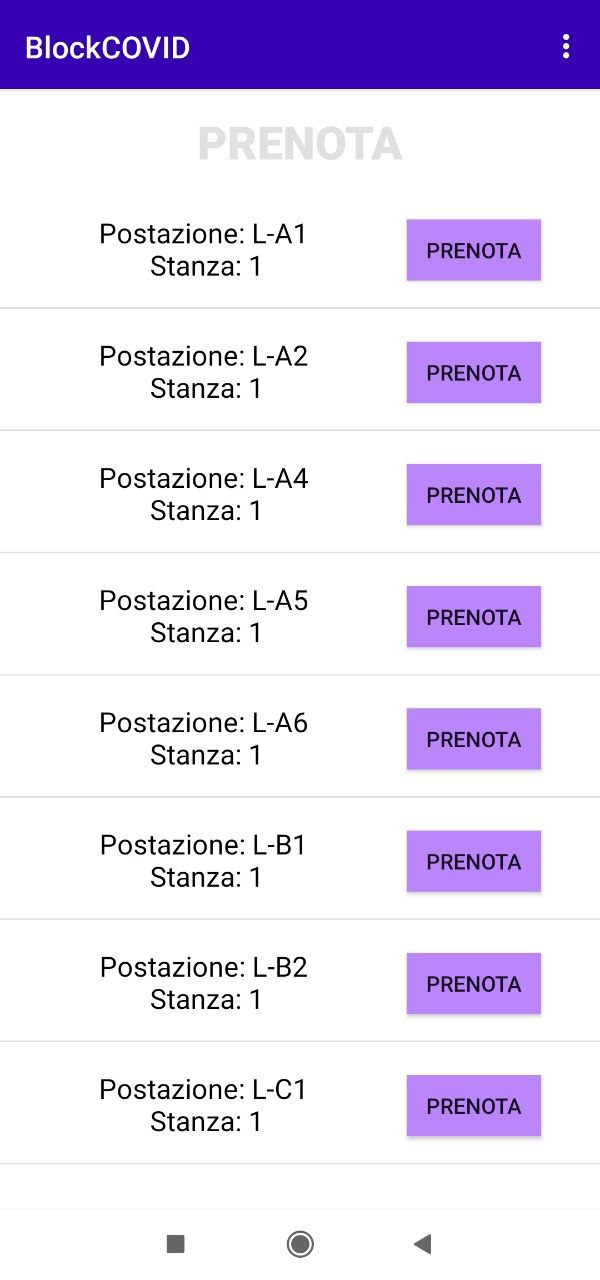
\includegraphics[width=5cm]{res/images/ListaPostazioniDaPrenotare.png}
		\caption{Lista postazioni prenotabili}
	\end{figure}
	
	
	\subsection{Utilizzo applicazione per gli addetti alle pulizie}
	L'applicazione mobile viene utilizzata dagli utenti che vogliono igienizzare una o più postazioni di una stanza dell'\glock{organizzazione}. 
	\\All'utente dell'applicazione vengono offerte tutte le funzionalità indicate in questa sezione.
	\subsubsection{Login}
	\begin{figure}[H]
		\centering
		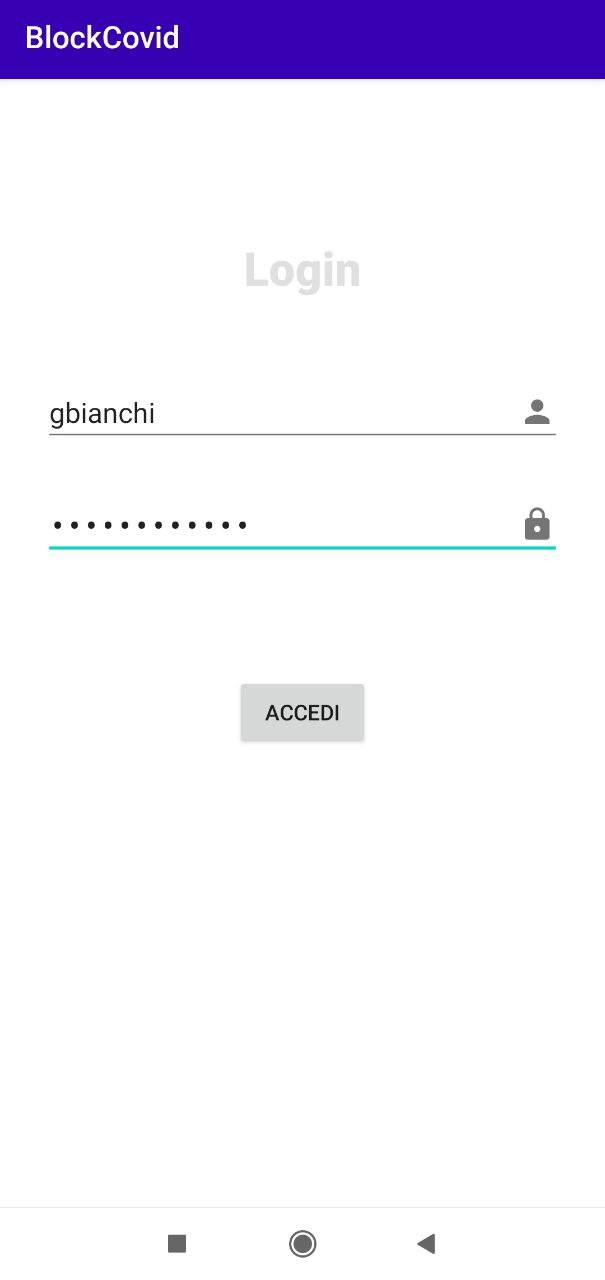
\includegraphics[width=5cm]{res/images/loginAddetto.png}
		\caption{Login utente}
	\end{figure}
	L'utente può autenticarsi nella pagina del login inserendo il proprio username e la propria password nelle caselle di testo corrispondenti.
	Nel caso in cui inserisca le credenziali corrette otterrà l'accesso all'applicazione e quindi alla pagina principale, altrimenti verrà visualizzato un messaggio di errore.
	\begin{figure}[H]
		\centering
		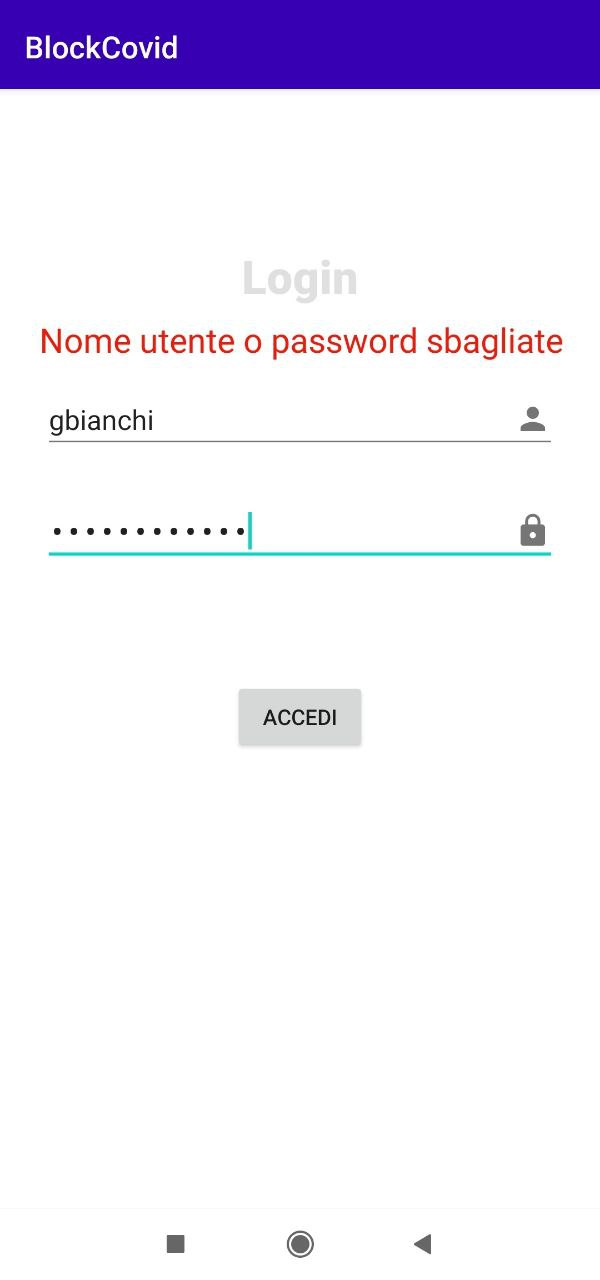
\includegraphics[width=5cm]{res/images/credenzialiErrateAddetto.png}
		\caption{Inserimento credenziali errate}
	\end{figure}
	
	\subsubsection{Logout}
	\begin{figure}[H]
		\centering
		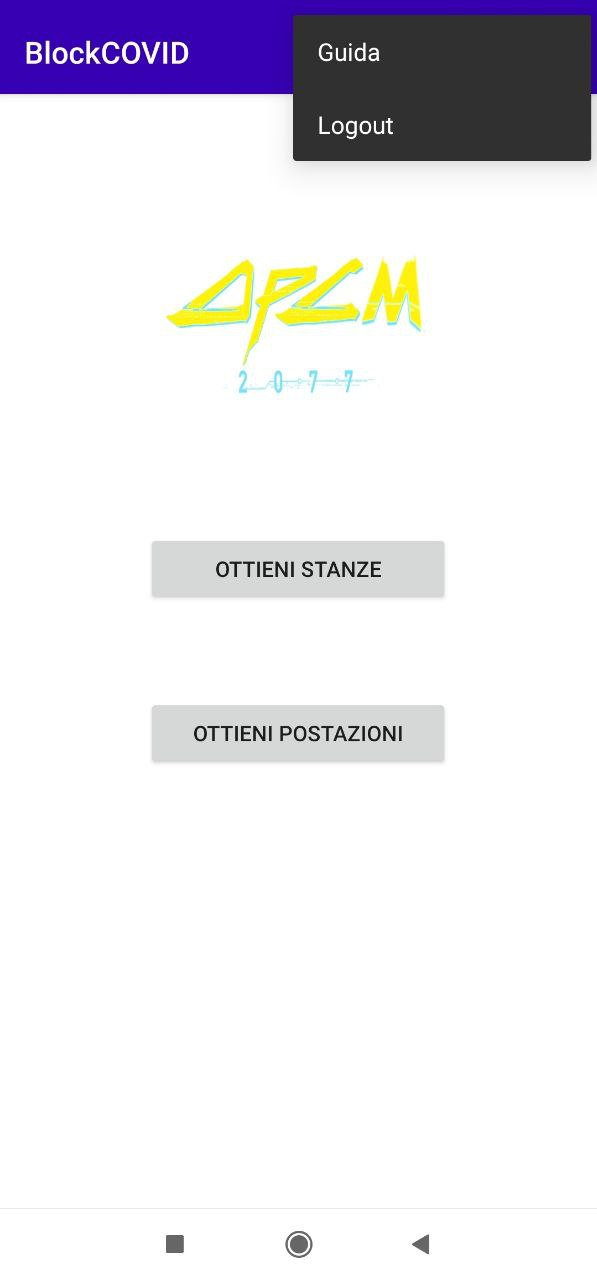
\includegraphics[width=5cm]{res/images/menuATendinaAddetto.png}
		\caption{Logout utente}
	\end{figure}
	L'utente può eseguire il logout aprendo il menù a tendina in alto a destra e poi cliccando su logout. Avvenuta questa operazione l'utente sarà deautenticato dal sistema e si troverà nella pagina del login.
	
	\subsubsection{Visualizzazione lista postazioni da igienizzare}
	\begin{figure}[H]
		\centering
		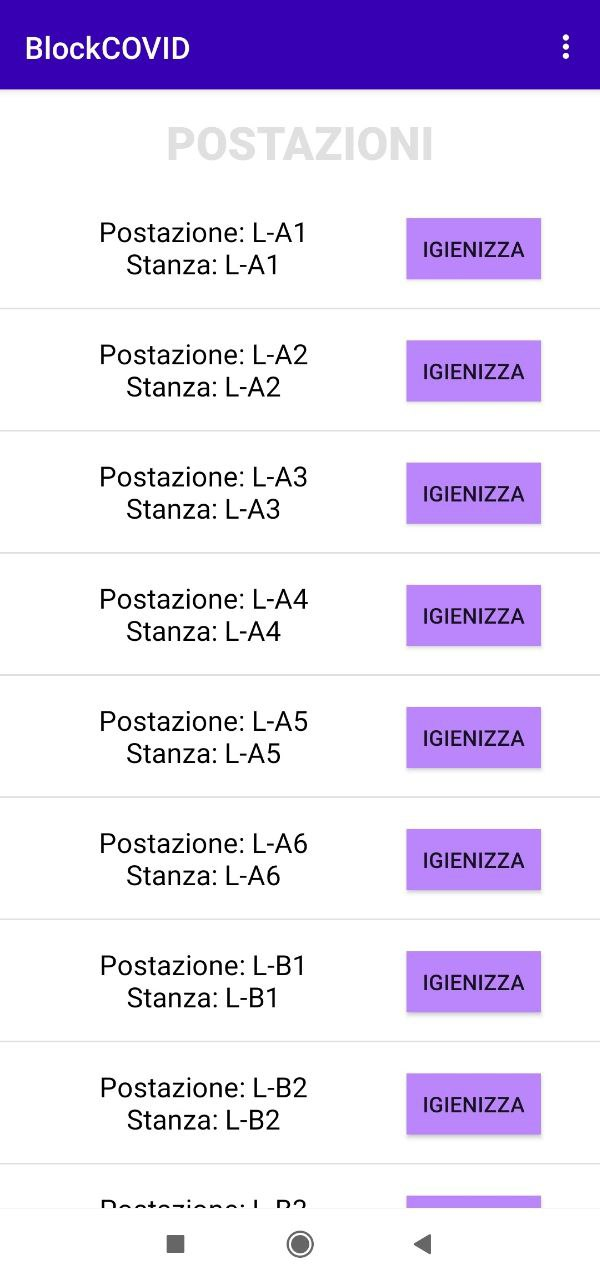
\includegraphics[width=5cm]{res/images/postazioniDaIgienizzareAddetto.png}
		\caption{Lista postazioni da igienizzare}
	\end{figure}	
	L’utente può accedere alla sezione per la visualizzazione della lista delle postazioni da igienizzare cliccando il bottone "Ottieni postazioni", presente nella pagina principale.
	Ogni postazione mostra le seguenti informazioni:
	\begin{itemize}
		\item nome della postazione;
		\item nome della stanza della postazione.
	\end{itemize}
	\subsubsection{Visualizzazione lista stanze da igienizzare}
	\begin{figure}[H]
		\centering
		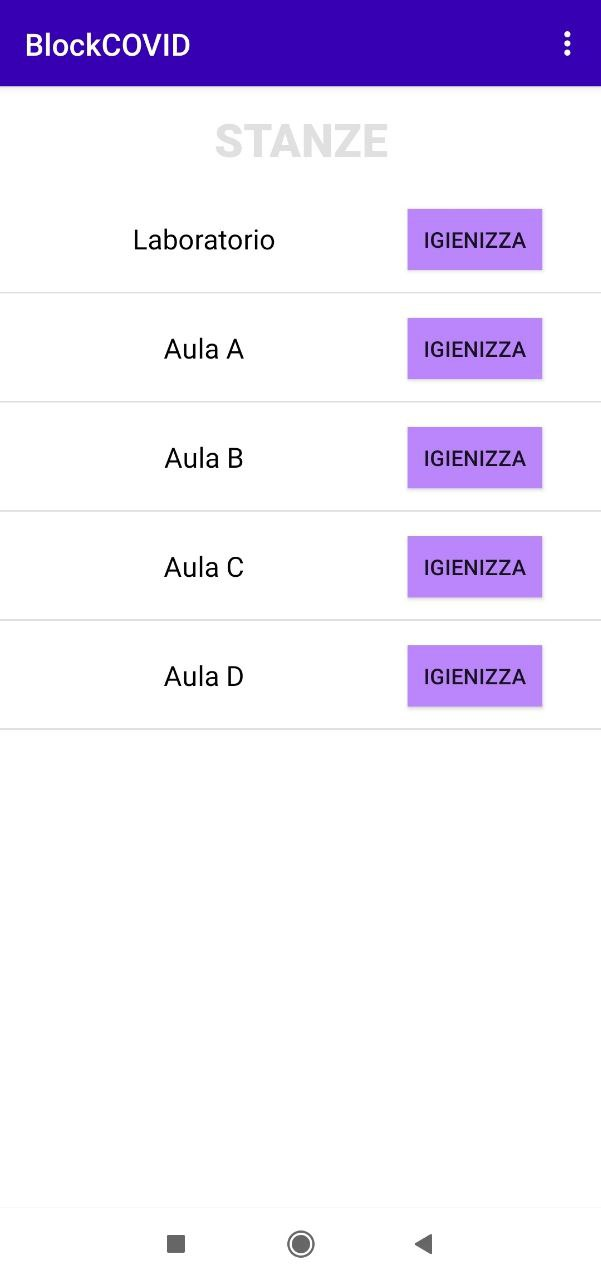
\includegraphics[width=5cm]{res/images/stanzeDaIgienizzareAddetto.png}
		\caption{Lista stanze da igienizzare}
	\end{figure}
	L’utente può accedere alla sezione per la visualizzazione della lista delle stanze da igienizzare cliccando il bottone "Ottieni stanze", presente nella pagina principale.
	Ogni stanza mostra come informazione il nome che la identifica.
	
	\subsubsection{Igienizzazione postazione}
	\begin{figure}[H]
		\centering
		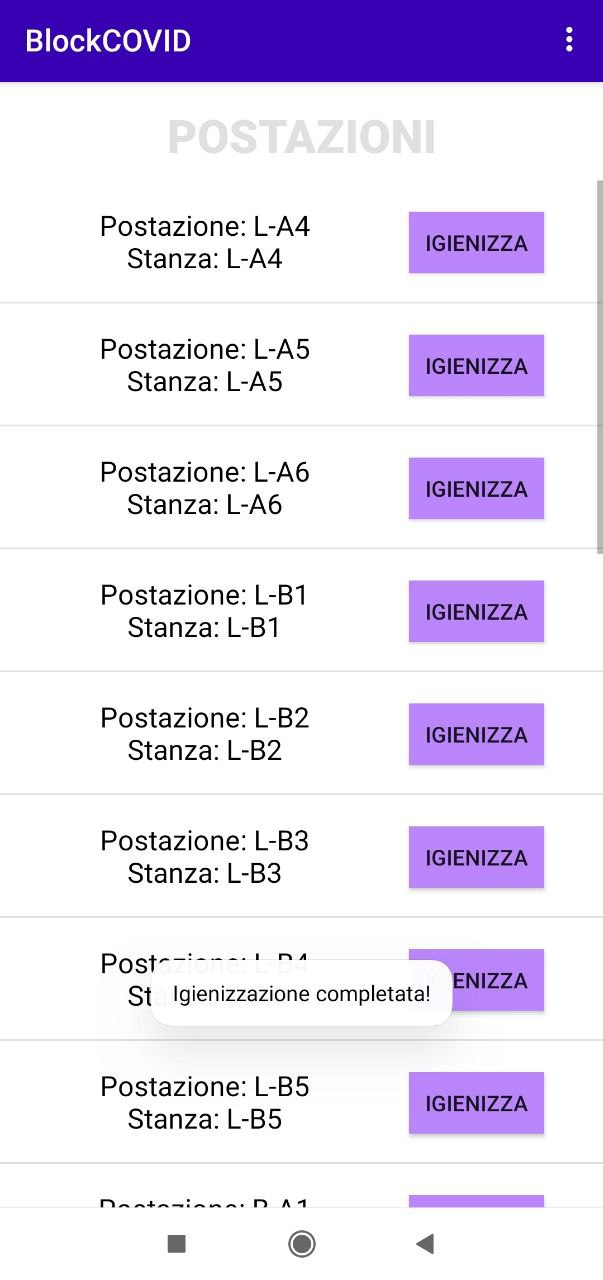
\includegraphics[width=5cm]{res/images/igienizzazionePostazioniAddetto.png}
		\caption{Postazione igienizzata}
	\end{figure}
	L'utente igienizza una postazione e lo segnala premendo l'apposito bottone "igienizza" presente sulla destra della postazione. In modo automatico la postazione igienizzata non verrà più visualizzata sulla lista e comparirà il messaggio "Igienizzazione completata!".
	
	\subsubsection{Igienizzazione stanza}
	\begin{figure}[H]
		\centering
		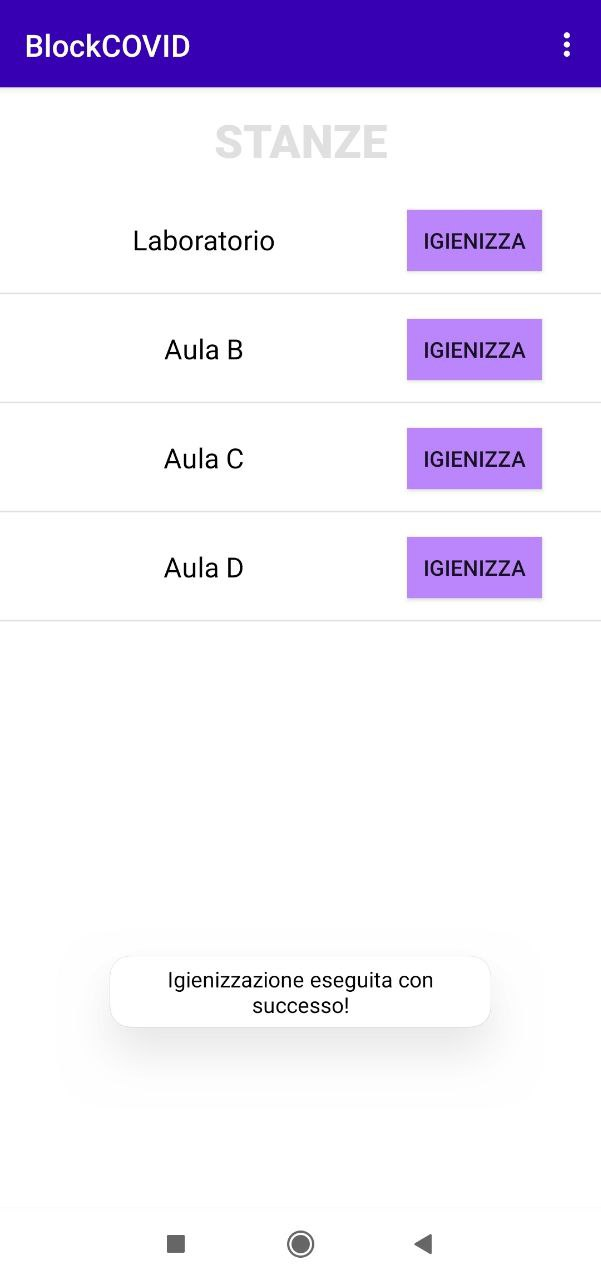
\includegraphics[width=5cm]{res/images/igienizzazioneStanza.png}
		\caption{Stanza igienizzata}
	\end{figure}
	L'utente igienizza una stanza e lo segnala premendo l'apposito bottone "igienizza" presente sulla destra della stanza. In modo automatico la stanza igienizzata non verrà più visualizzata sulla lista e comparirà il messaggio "Igienizzazione eseguita con successo!".
	\subsubsection{Guida utente}
	\begin{figure}[H]
		\centering
		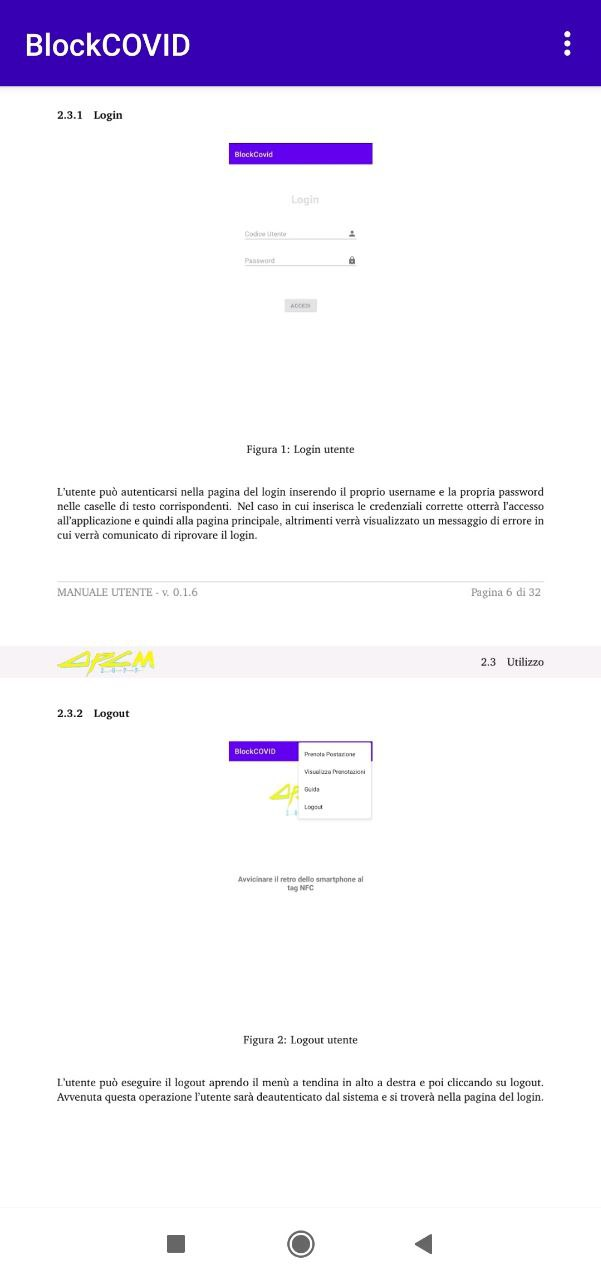
\includegraphics[width=5cm]{res/images/guidaAddetto.png}
		\caption{Guida addetto alle pulizie}
	\end{figure}
	L’utente accede alla pagina "Guida utente", cliccando la sezione apposita del menù a tendina in alto a destra, e riceve una guida riguardo le funzionalità principali dell'applicazione.
	
	 
	
	
